\section{Restoration, Revival, Renaissance}

\begin{wrapfigure}{rt}{.3\textwidth}
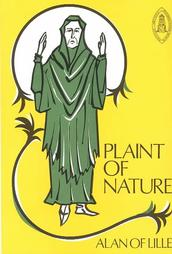
\includegraphics[width=.3\textwidth]{plaint-nature-alain-de-lille-paperback-cover-art.jpg}
\end{wrapfigure}

The order of these nouns is deliberate. Secular humanists desire to have the last without either of the first two, particularly and most insistently, the first. Christians are generally unconcerned or even aware of the first, \& if it is brought to their attention, they become truculent. The third also escapes the notice of many of them, who have been relegated to the merchant or warrior castes, or who have been converted while being laborers or even \emph{shudras}. In fact, one of the primary dogmas of this era is the idea (variously expressed) that ``you can't go back'', that ``(all) change is good'', \& that ``new is always better'', and almost no one dissents from it. (Wendell Berry hilariously points out\footnote{\url{http://www.jesusradicals.com/wp-content/uploads/computer.pdf}} that if using a computer is a new idea, then not using one is an even ``more novel'' one.)

\textbf{\emph{That is why it is important to pursue one's vocation and caste, as well as practice the ``lesser mysteries}}``, rather than spend too much time worrying if one has attained supreme Enlightenment. Because in the New Age worldview, to not have reached the summit of Mount Parnassus is to not have done anything. This reminds one of A. Jarry's evil motto -- ``\emph{Until we've destroyed everything, we haven't done anything}``. This bastard-like, ungrateful, and rebellious attitude has transferred itself out of the failed 60's movements, \& into the ``mainstream''. Nowadays, if someone doesn't have visions of the angels, adopt children from foreign countries, and float through life in a haze of super-tolerance and up-to-date information, then why possibly bother? Beware of thinking like those who are masterless and rebellious.

Tracy Lee Simmons points out in \emph{Climbing Mount Parnassus}\footnote{\url{http://www.amazon.com/Climbing-Parnassus-Apologia-Greek-Latin/dp/1933859504}} that

\begin{quotex}
The foundations of the modern world are viewed more competently from this (the ``classics'': study of Greek/Roman civilization) height. Poetry, drama, democracy, idealism, scientific curiosity, and so much else furnishing our minds are better grasped, and better judged. We drift without classics, floating on our own deracinated, exiguous islands. And we become fodder for demagogues. We need not a revolution, but a restoration.
\end{quotex}


I will give you an example. Alcibiades, in Thucydides' \emph{History}, defines democracy as the concern simply that the good of all be given due consideration, rather than merely the good of a few (the non-slaves). Now Alcibiades was bargaining for his life with the Spartans, to whom he had fled in exile, so perhaps he was being disingenuous. Nevertheless, even the villains and knaves of ancient history have an unpolished grace that should make us blush. Jose Maria Gironella in \emph{The Cypresses Believe in God}, has Ignatio say that he defines socialism as the belief that the ``rich shouldn't have everything, and the poor nothing''. Rather than hate democracy uncategorically, perhaps it would be better to examine it \& to see where it legitimately applies (eg., local self-governance) \& where it becomes an ersatz religion, a demon, and a false God.

In the context of real Restoration, of that which is always True \& is always so \& abides forever, a great many false dichotomies and catch phrases dissolve into clarity. GK Chesterton, for instance, attempts in his Agrarian and Distributionist thought (which he bases on Hillaire Belloc and other Catholic thinkers), to demonstrate what ``Christian democracy'' actually meant, rather than what it came to mean detached from God, the soil, and all wisdom.

Therefore, the first thing or first question is ``what constitutes Restoration''? As Jacques Barzun notes of education, it is dangerous to look too closely at the object (like staring at the sun, or trying to see the Pleiades head on), because the growth of ``education'' (or Restoration) is a slow, intangible, and subtle process which is difficult to assess. It might be better, argues Barzun, to stick to teaching Latin, Greek, chemistry, and the rest of the traditional subjects well (just a few of them), and let ``education'' occur like the growth of a tree. So, work at the destined work of your vocation; practice what lesser mysteries Providence brings to your attention; \& assiduously and patiently cultivate your spiritual garden. You are climbing Mount Parnassus\footnote{\url{http://en.wikipedia.org/wiki/Mount\_Parnassus}}.

If one is drinking from the fountain of Tradition (which can be increasingly recognized the more and deeper draughts one imbibes), then you need not fear to lose the way. Alain de Lille (doctor universalis, d. 1203) wrote of the ``intelligible sphere whose center is everywhere, and whose circumference is nowhere'' because he had drunk from it. And where did he find such wisdom? Of course, first of all, he had read or been told of such a hermetic tradition. Yet also, it is said that he was preparing a lecture on the attributes of God, and had gone down to the Seine River bank to walk. He met a young child, who had dug a hole in the sand. The teacher told the boy he was lecturing on God tomorrow, and asked what he was doing. The child said, ``I am putting the river inside of this hole''. The doctor laughed heartily, and said there was no possibility of that, that his purpose would fail. The boy looked at him, and said that it would be equally impossible to speak of God the next morning. Alanus\footnote{\url{http://www.princeton.edu/\~achaney/tmve/wiki100k/docs/Alain\_de\_Lille.html}} was shattered, and although he showed up the next morning, he tore his robe off, \& without another word, strode out of the university to join a monastery and find the answer to the riddle. God will speak to you in homely terms, in the lesser mysteries, in exoteric religion or philosophy, as surely as in the greatest terms, \& the Christians assert that this is due to the Incarnation.

Incidentally, for Christian readers, I will recommend Coleston Brown's \emph{Magical Christianity}\footnote{\url{http://www.amazon.com/Magical-Christianity-Symbols-Spiritual-Meditations/dp/0835608557}} (the source of the Alanus de Lille story) as a sourcebook for uncovering the Tradition hidden within their own religion. It matches well with Iamblichus' progression of the first ten numbers, and we shall see if it has any correspondence with the zodiac of Hercule's labors, as well.


\flrightit{Posted on 2013-11-23 by Logres}

